% This work is licensed under
% http://creativecommon.org/licenses/by/3.0/
\section{Examples of session-location mobility}
\label{sec:sec6}

In this section we compare four proposals for session-location
mobility: the
Host Identity Protocol (HIP)~\cite{RFC-4423,HIP}, 
the Identifier-Locator Network Protocol (ILNP) \cite{ILNP1,ILNP2},
the
Locator/Identifier Separation Protocol (LISP) Mobile Node~\cite{LISP-MN}, 
and the ``route optimization'' mechanism of Mobile 
IPv6 \cite{mipv6old,mipv6new}
(Section~\ref{sec:mipv6} will explain how route optimization fits into
Mobile IPv6 overall).
All but ILNP are IETF standards, and ILNP has resulted in many
IETF documents with ``experimental'' status.

These proposals have many similarities, as
they all provide mobility by splitting 
the Internet core layer (shown in Figure~\ref{fig:scope}) into two
layers.
These two layers 
are shown in Figure~\ref{fig:identloc}, and also correspond to
the two layers in Figure~\ref{fig:slm}.
SLM supports the persistence of inter-layer channels that are
links in the upper layer and sessions in the lower
layer.\footnote{Note that the members of the
identifier layer are {\it hosts}, while the members of the locator
layer are {\it interfaces}.
This distinction can safely be ignored in this section, but it is
important for multihoming as discussed in Section~\ref{sec:multihoming}.}

\begin{figure}
\centering
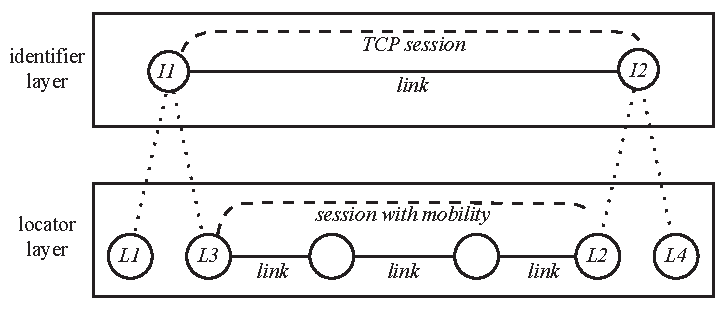
\includegraphics[scale=0.80]{figures/identloc.pdf}
\caption{The Internet core layer splits into two layers for
well-known examples of session-location mobility.  
In the identifier layer, session protocols such as TCP run
largely unmodified.
In the locator layer, the session protocol implements mobility.}
\label{fig:identloc}
\end{figure}

In an attempt to use a widely acceptable common terminology,
we call the upper layer 
the {\it identifier layer}, and the lower layer
the {\it locator layer}.
Names in the two layers are referred to as {\it identifiers} and
{\it locators}, respectively.
This common terminology does not necessarily match the terminology
typically used to explain each specific protocol.

Note that
Figure~\ref{fig:identloc} is an approximation of the real
implementations of these standards, in which the split between layers may
be implicit or incomplete.
In the geomorphic view, two separate session protocols are employed.
In the identifier layer, a largely unmodified TCP implementation provides
the usual TCP service as if identifiers were IP addresses.
(UDP and other service protocols operate here 
as well.)
In the locator layer, the only purpose of the session protocol is
to implement SLM.

\subsection{Names}

Table~\ref{tab:slm} compares the four proposals on their choices of
names.
They differ most on identifiers, which must be globally unique and
persistent, but have no other necessary constraints.

\begin{table}
\begin{center}
\footnotesize
\begin{tabular}{|l|l|l|} \hline
\multicolumn{1}{|c|}{\bf Protocol} & 
  \multicolumn{1}{c|}{\bf Identifier} & 
  \multicolumn{1}{c|}{\bf Locator} \\ \hline
HIP & (hash of) public key & IPv4 or IPv6 address \\ \hline
ILNPv6 & 64-bit IPv6 suffix & IPv6 address \\ \hline
LISP Mobile Node & IPv4/IPv6 address (called EID) & IPv4/IPv6 address (called RLoc) \\ \hline
Mobile IPv6 & IPv6 address & IPv6 address \\ \hline
\end{tabular}
\end{center}
\caption{Comparison of SLM proposals on the basis of names.}
\label{tab:slm}
\end{table}

HIP places a great emphasis on building in security, so the identifier
of a host is the host's
public cryptographic key.
With the use of keys as identifiers, 
messages can have self-authenticating source information.
Self-authentication provides security within the SLM locator
update protocol (see Section~\ref{sec:updateprotocols}), while
the guaranteed presence of a public key makes it easy to protect
the channel data with encryption.
Identifiers can also be hashes of public keys, which allows for shorter
identifiers without sacrificing self-authentication.

ILNPv6 is the IPv6 version of ILNP.
Its identifiers are 64 bits long; a host usually chooses a unique
identifier for itself
by taking the 48-bit MAC address of one of its hardware
interfaces and using a standard algorithm to extend it to 64 bits.

The significance of 64 bits is that in IPv6 routing based on 
hierarchical names and aggregation, the longest possible prefix is
64 bits.
This means that at its finest-grained, IPv6 routing examines the
first 64 bits of an IPv6 address and points to a
subnetwork.
The IPv6 address still has a 64-bit suffix to map to an IPv6 interface
attached to the subnetwork.
In ILNPv6, 
identifiers are carried in the 64-bit suffixes of IPv6 addresses.
In other words, an ILNPv6 locator is derived from an ILNPv6 identifier
by prefixing 64 bits that indicate a subnetwork where the identified
host can be found.\footnote{This is different from ILNP terminology,
in which the 64-bit prefix is itself the ``locator.''} 
This scheme is very efficient in its use of address bits.

By basing identifiers on MAC addresses, which are globally unique,
ILNP ensures that hosts have unique identifiers without relying on any
administrative authority.
ILNP requires that, when a host joins a new subnetwork, it is allowed
to choose its own 64-bit address suffix.

LISP Mobile Node and Mobile IPv6 are less interesting.
In both cases, identifiers are normal routable IP addresses.

Naming choices have the biggest effect on the deployment opportunities
of a design.
Mobile IPv6 requires the deployment of IPv6.
HIP and ILNP require more changes to TCP because their identifiers
are not IP addresses.
Deployment of new protocols is usually incremental, which means
that upgraded hosts and subnetworks must interoperate with legacy
hosts and subnetworks.
This raises the following interesting question: if an IP-based
SLM protocol is interoperating with ordinary IP, does the ordinary Internet
layer coincide with the identifier layer or the locator layer?
Interoperation will work best if the ordinary Internet layer 
coincides with the identifier layer.
This composition of layers (making the SLM identifier layer and Internet
layer into one) will work best if SLM identifiers look like ordinary
IP addresses.

\subsection{Directories}

An implementation of SLM requires a globally accessible
implementation of {\it locations} in the locator layer, mapping 
identifiers to locators.
Table~\ref{tab:slm2} compares the four standards on their choices of
location directory or other mapping implementation.

\begin{table}
\begin{center}
\footnotesize
\begin{tabular}{|l|l|} \hline
\multicolumn{1}{|c|}{\bf Protocol} & 
  \multicolumn{1}{c|}{\bf Location Directory} \\ \hline 
HIP & DNS \\ \hline
ILNP & DNS \\ \hline
LISP Mobile Node & LISP subsystem \\ \hline
Mobile IPv6 & home agent for each host has its locator  \\ \hline
\end{tabular}
\end{center}
\caption{Comparison of SLM proposals on the basis of directories.}
\label{tab:slm2}
\end{table}

LISP Mobile Node inherits its directory mechanism from LISP \cite{LISP},
which is an IETF standard designed for a different purpose 
(multihoming of large-scale enterprise subnetworks), and not
originally intended for the support of mobility.
The directory mechanism is a special-purpose distributed subsystem
of directory servers.
While this requires a substantial initial investment, it does give
the deployer maximum freedom.
For example, different deployments could use almost any name space
as the set of identifiers.
 
Both HIP and ILNP usually make use of the Domain Name System (DNS) as a
scalable, highly available directory subsystem.
When they do, note that their use of DNS is different from the
ordinary use of DNS, which is to map application-level names
(domain names) to IP addresses (which, as we have seen, can sometimes
be interpreted as identifiers or locators).
An IP-oriented SLM mechanism requires a directory or the equivalent to map
IP-oriented
identifiers to IP-oriented
locators, which has nothing inherently
to do with application-level names.

DNS relies on the hierarchical structure of domain names both
for scalability of lookups and to manage the distributed
administration of DNS servers.
Consequently, a DNS lookup must begin with a domain name.
Thus when HIP and ILNP use DNS as their directory subsystem,
every mobile host must have a domain name that serves as a key for 
finding its current location, even though the domain name is not
in the name space of either of the relevant layers, and may not be
needed for any other reason.
For example, in the use of a client-server service, 
the server usually has a domain name while the client does not.
But if the client is mobile with HIP or ILNP, it must have a domain
name, known to the server, for this purpose alone.

For both HIP and ILNP
it is necessary to add new record types to those stored
by DNS servers, because the value being looked up is not always an
IP address.
Finally, the DNS server with 
the authoritative copy of a locator must send it out with
a small time-to-live, preferably zero.
Otherwise other DNS servers 
will cache the information for longer times, 
impeding responsiveness to changes of location.

The route optimization (SLM) 
mechanism of Mobile IPv6 is an adjunct to the Mobile IPv6
DRM implementation (see Sections~\ref{sec:mipv4} and \ref{sec:mipv6}).
Because the DRM implementation uses home agents, the SLM implementation
uses them also.
The current locator of an identifier can always be obtained from its
home agent.
Mobile IPv6 may be less reliable than other designs because 
a home agents is a single point of failure with respect to its
mobile hosts.
Home agents do not necessarily have the built-in redundancy and
high availability that the directories of the other designs have.

\subsection{Locator update protocols}
\label{sec:updateprotocols}

An implementation of SLM must have a protocol through which 
mobile nodes update the directory and their correspondents after
a move.
The protocol must have security to prevent updates from unauthorized
hosts.

It would take far too much space to report on how each proposal
meets these requirements.
Also, many standards provide a menu of implementation alternatives,
some of them better-documented than others.
In lieu of this detail, 
we will merely touch on a few of the design issues for SLM
protocols.

Even without the problem of simultaneous handoff (as introduced in
Section~\ref{sec:slm}), an update protocol can suffer from lost
or re-ordered messages.
If a correspondent node or directory
receives two different update messages from a
mobile host in the wrong order, it could retain an obsolete locator
for the mobile node.
If a correspondent node or directory
determines from sequence numbers that an
update message has been lost, it might wait forever for a retransmission
that will not come because the mobile node is somewhere else and will
not receive the retransmission request.
These bugs have been discovered in real SLM protocols \cite{serval-icnp}.
In general, the two techniques to rely on are (1) version numbers
rather than sequence numbers, and (2) some form of protocol verification
to insure against otherwise-almost-inevitable mistakes.

If an endpoint loses track of the session's other endpoint because
of simultaneous handoff, loss of update messages, or a protocol bug,
it can always get the current locator by making a new lookup
in the directory.
In general, an SLM protocol can be made more robust by having mobile
nodes report their locators to the directory frequently,
and having correspondent nodes refresh their cached locators
from the directory frequently.
This robustness comes at the cost of increased overhead in the
form of message traffic.

HIP uses a different method to solve the problem of simultaneous handoff.
When a mobile host moves, its old locator is adopted by a
``rendezvous server'' that keeps track of its new locator.
The rendezvous server intercepts control messages destined for the
old locator, and forwards them to the new locator.
Even when both endpoints of a session move at the same time,
their update messages will reach each other through rendezvous servers.
As always, data messages travel directly between hosts.

\subsection{Encapsulation}

Like Table~\ref{tab:overlays},
Table~\ref{tab:slm3} compares the standards on the basis of
how they encapsulate overlay messages as they travel through an
underlay.
Note that there are two versions of the Mobile IPv6 standard which
differ in this respect (the newer \cite{mipv6new} supersedes the 
older \cite{mipv6old}, so this
comparison is of academic interest only).

\begin{table}
\begin{center}
\footnotesize
\begin{tabular}{|l|l|} \hline
\multicolumn{1}{|c|}{\bf Protocol} & 
  \multicolumn{1}{c|}{\bf Encapsulation} \\ \hline 
HIP & encapsulation with IPSec Encapsulating Security Payload \\ \hline
ILNPv6 & none, identifier is extracted from locator \\ \hline
LISP Mobile Node & simple encapsulation \\ \hline
Mobile IPv6 (RFC 3775) & simple encapsulation  \\ \hline
Mobile IPv6 (RFC 6275) & Home Address destination option and Type 2 Header  \\ \hline
\end{tabular}
\end{center}
\caption{Comparison of SLM proposals on the basis of encapsulation.}
\label{tab:slm3}
\end{table}

Consider a message being sent from left to right in 
Figure~\ref{fig:identloc}, at a time when identifier
{\it I1} has locator {\it L3} and identifier {\it I2} has
locator {\it L2}.
In the simplest implementation, the message consists of a message
with source {\it I1} and destination {\it I2}, encapsulated
in a message with 
source {\it L3} and destination {\it L2}.
There are other possibilities, however, motivated by the desire
to conserve space in message headers.
This is a serious concern in IPv6, where each of the four address
fields is 128 bits long.

LISP Mobile Node and the original version of Mobile IPv6 use simple
encapsulation as above.
HIP does also, with the additional proviso that the message body
containing the identifiers is protected with IPsec.
In ILNP each identifier is a suffix of its current locator, so it
need not be sent separately.

In the revised Mobile IPv6 standard, there is an optimization 
apparently based on the observation that, most of the time, only
one of the endpoints of a session will be mobile.
For a stationary node, the identifier and locator are always the
same, and need not be sent twice.
So a message from the mobile node needs a source identifier and
not a destination identifier, and a message to a mobile node
needs a destination identifier and not a source identifier.

Now let us assume that {\it I1} is mobile and {\it I2} is stationary.
For messages from {\it I2} to {\it I1}, a destination identifier is 
needed.
The revised Mobile IPv6 standard uses
a special Type~2 header.
This is a kind of ``source routing'' header, allowing the source to
provide a list of destination
addresses through which the message must be routed.
The messages have destination list ({\it L3; I1}), where the second
hop from {\it L3} to {\it I1} is internal to the mobile host.
For messages from {\it I1} to {\it I2}, a source identifier is needed.
The extra source address {\it I1} is inserted using a special
``Home Address destination option.''
This option is an extension to IPv6 allowing an extra field in a
message header.
In this way, the extra identifiers can be added to messages only when
needed.

One might speculate that such a complex optimization would cause
trouble in the form of further, cascading complexities,
and this is indeed the case.
There are elaborate rules in \cite{mipv6new} for processing
messages so that IPsec works correctly:
each message must be processed partially with {\it I1} in the ordinary
source or destination field, and partially with {\it I1} moved to the
Type 2 header or Home Address destination option field.
Note that this is an interaction that has been explicitly recognized
and accommodated in the standard.
No one knows how many problematic interactions with other protocols,
caused by this optimization,
will be discovered if Mobile IPv6 comes into widespread use.

The SLM implementation of Mobile IPv6 is constrained by the need to
compose with the DRM implementation of Mobile
IPv6 (see Section~\ref{sec:mipv6}).
If there were not so many constraints,
the size of
headers could be reduced without violating the principle of separation
of concerns.
For example, Figure~\ref{fig:identloc2} revises
Figure~\ref{fig:identloc} in an obvious way as suggested by the
geomorphic view.
The session protocol in the locator layer now performs both TCP and SLM
functions.

\begin{figure}
\centering
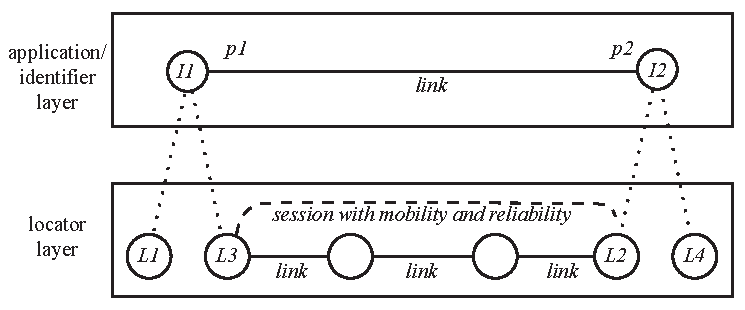
\includegraphics[scale=0.80]{figures/identloc2.pdf}
\caption{A more efficient version of Figure~\ref{fig:identloc}.}
\label{fig:identloc2}
\end{figure}

In the identifier layer, the link between {\it I1} and {\it I2}
is uniquely identified at one end by {\it I1, p1}, where {\it p1}
is a port number, and uniquely identified at the other end by
{\it I2, p2}.
Note that
the identifier layer is more like an application layer than an IP
layer in that it has no forwarding---only direct links between pairs
of communicating endpoints.
Consequently, once the link has been set up, there is absolutely
no need to transmit {\it I1} and {\it I2} in data messages.
Each endpoint simply uses the port number to pass messages unambiguously
across the layer boundary.
Figure~\ref{fig:identloc2} has many similarities with TCP Migrate
\cite{tcp-migrate} and Serval \cite{serval,serval-icnp}, which are other
proposals for SLM.
